% questions.tex —— 2008 年·全国大纲卷Ⅱ·文科 · 题目内容片段（无答案）
% 由 tools/generate_projects.py 依来源总账自 2008/2008_数学真题_全国2文_试题.md 生成，勿手改（改源 MD 后重跑）


\gkpart{数学}

\begin{gktip}
\textbf{来源说明}：本题面依据固定源 PDF 两页 A3 题面逐题转录，原卷印刷页码 439–440。固定源不附答案，答案和解析均由本库独立复算。

\textbf{图形说明}：第 20 题的原卷图形关系重绘为 TikZ/PGFPlots 矢量图。图形标记所指的 PNG 不随仓库保存。
\end{gktip}

\gkpart{一、选择题}

\begin{question}
\gkti{1}若 $\sin\alpha<0$ 且 $\tan\alpha>0$，则 $\alpha$ 是\mbox{（　　）}

（A）第一象限角\quad（B）第二象限角\quad（C）第三象限角\quad（D）第四象限角

\end{question}
\begin{question}
\gkti{2}设集合 $M=\{m\in\mathbb Z\mid-3<m<2\}$，$N=\{n\in\mathbb Z\mid-1\leqslant n\leqslant3\}$，则 $M\cap N=$\mbox{（　　）}

（A）$\{0,1\}$\quad（B）$\{-1,0,1\}$\quad（C）$\{0,1,2\}$\quad（D）$\{-1,0,1,2\}$

\end{question}
\begin{question}
\gkti{3}原点到直线 $x+2y-5=0$ 的距离为\mbox{（　　）}

（A）$1$\quad（B）$\sqrt3$\quad（C）$2$\quad（D）$\sqrt5$

\end{question}
\begin{question}
\gkti{4}函数 $f(x)=\dfrac1x-x$ 的图象关于\mbox{（　　）}

（A）$y$ 轴对称\quad（B）直线 $y=-x$ 对称\quad（C）坐标原点对称\quad（D）直线 $y=x$ 对称

\end{question}
\begin{question}
\gkti{5}若 $x\in(e^{-1},1)$，$a=\ln x$，$b=2\ln x$，$c=\ln^3x$，则\mbox{（　　）}

（A）$a<b<c$\quad（B）$c<a<b$\quad（C）$b<a<c$\quad（D）$b<c<a$

\end{question}
\begin{question}
\gkti{6}设变量 $x,y$ 满足约束条件

\nopagebreak[4]
\[
\begin{cases}
y\geqslant x,\\
x+2y\leqslant2,\\
x\geqslant-2,
\end{cases}
\]

则 $z=x-3y$ 的最小值为\mbox{（　　）}

（A）$-2$\quad（B）$-4$\quad（C）$-6$\quad（D）$-8$

\end{question}
\begin{question}
\gkti{7}设曲线 $y=ax^2$ 在点 $(1,a)$ 处的切线与直线 $2x-y-6=0$ 平行，则 $a=$\mbox{（　　）}

（A）$1$\quad（B）$\dfrac12$\quad（C）$-\dfrac12$\quad（D）$-1$

\end{question}
\begin{question}
\gkti{8}正四棱锥的侧棱长为 $2\sqrt3$，侧棱与底面所成的角为 $60^\circ$，则该棱锥的体积为\mbox{（　　）}

（A）$3$\quad（B）$6$\quad（C）$9$\quad（D）$18$

\end{question}
\begin{question}
\gkti{9}$(1-\sqrt{x})^4(1+\sqrt{x})^4$ 的展开式中 $x$ 的系数是\mbox{（　　）}

（A）$-4$\quad（B）$-3$\quad（C）$3$\quad（D）$4$

\end{question}
\begin{question}
\gkti{10}函数 $f(x)=\sin x-\cos x$ 的最大值为\mbox{（　　）}

（A）$1$\quad（B）$\sqrt2$\quad（C）$\sqrt3$\quad（D）$2$

\end{question}
\begin{question}
\gkti{11}设 $\triangle ABC$ 是等腰三角形，$\angle ABC=120^\circ$，则以 $A\text{、}B$ 为焦点且过点 $C$ 的双曲线的离心率为\mbox{（　　）}

（A）$\dfrac{1+\sqrt2}{2}$\quad（B）$\dfrac{1+\sqrt3}{2}$\quad（C）$1+\sqrt2$\quad（D）$1+\sqrt3$

\end{question}
\begin{question}
\gkti{12}已知球的半径为 $2$，相互垂直的两个平面分别截球面得两个圆。若两圆的公共弦长为 $2$，则两圆的圆心距等于\mbox{（　　）}

（A）$1$\quad（B）$\sqrt2$\quad（C）$\sqrt3$\quad（D）$2$

\end{question}
\gkpart{二、填空题}

\begin{question}
\gkti{13}设向量 $\boldsymbol a=(1,2)$，$\boldsymbol b=(2,3)$。若向量 $\lambda\boldsymbol a+\boldsymbol b$ 与向量 $\boldsymbol c=(-4,-7)$ 共线，则 $\lambda=$\gkblank{}。

\end{question}
\begin{question}
\gkti{14}从 $10$ 名男同学、$6$ 名女同学中选 $3$ 名参加体能测试，则选到的 $3$ 名同学中既有男同学又有女同学的不同选法共有\gkblank{}种。（用数字作答）

\end{question}
\begin{question}
\gkti{15}已知 $F$ 是抛物线 $C:y^2=4x$ 的焦点，$A\text{、}B$ 是 $C$ 上的两个点，线段 $AB$ 的中点为 $M(2,2)$，则 $\triangle ABF$ 的面积等于\gkblank{}。

\end{question}
\begin{question}
\gkti{16}平面内的一个四边形为平行四边形的充要条件有多个，如两组对边分别平行。类似地，写出空间中的一个四棱柱为平行六面体的两个充要条件：充要条件①\gkblank{}；充要条件②\gkblank{}。（写出你认为正确的两个充要条件）

\end{question}
\gkpart{三、解答题}

\begin{question}
\gkti{17}在 $\triangle ABC$ 中，$\cos A=-\dfrac5{13}$，$\cos B=\dfrac35$。

（1） 求 $\sin C$ 的值；

（2） 设 $BC=5$，求 $\triangle ABC$ 的面积。

\end{question}
\begin{question}
\gkti{18}等差数列 $\{a_n\}$ 中，$a_4=10$，且 $a_3\text{、}a_6\text{、}a_{10}$ 成等比数列。求数列 $\{a_n\}$ 前 $20$ 项的和 $S_{20}$。

\end{question}
\begin{question}
\gkti{19}甲、乙两人进行射击比赛，在一轮比赛中，甲、乙各射击一发子弹。根据以往资料知，甲击中 $8$ 环、$9$ 环、$10$ 环的概率分别为 $0.6,0.3,0.1$，乙击中 $8$ 环、$9$ 环、$10$ 环的概率分别为 $0.4,0.4,0.2$。设甲、乙的射击相互独立。

（1） 求在一轮比赛中甲击中的环数多于乙击中环数的概率；

（2） 求在独立的三轮比赛中，至少有两轮甲击中的环数多于乙击中环数的概率。

\Needspace{0.4\textheight}
\end{question}
\begin{question}
\gkti{20}如图，正四棱柱 $ABCD-A_1B_1C_1D_1$ 中，$AA_1=2AB=4$，点 $E$ 在 $CC_1$ 上且 $C_1E=3EC$。
\nopagebreak[4]
\begin{center}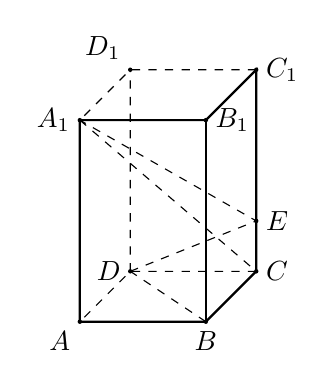
\begin{tikzpicture}[scale=.8,>=stealth]
\coordinate (A) at (0,0); \coordinate (B) at (2,0);
\coordinate (C) at (2.8,.8); \coordinate (D) at (.8,.8);
\coordinate (A1) at (0,3.2); \coordinate (B1) at (2,3.2);
\coordinate (C1) at (2.8,4); \coordinate (D1) at (.8,4);
\coordinate (E) at (2.8,1.6);
\draw[thick] (A)--(B)--(C)--(C1)--(B1)--(A1)--cycle;
\draw[dashed] (C)--(D)--(A) (C1)--(D1)--(A1) (D)--(D1);
\draw[thick] (B)--(B1) (C)--(C1);
\draw[dashed] (A1)--(C) (B)--(D) (D)--(E)--(A1);
\fill (A) circle (1pt) node[below left] {$A$};
\fill (B) circle (1pt) node[below] {$B$};
\fill (C) circle (1pt) node[right] {$C$};
\fill (D) circle (1pt) node[left] {$D$};
\fill (A1) circle (1pt) node[left] {$A_1$};
\fill (B1) circle (1pt) node[right] {$B_1$};
\fill (C1) circle (1pt) node[right] {$C_1$};
\fill (D1) circle (1pt) node[above left] {$D_1$};
\fill (E) circle (1pt) node[right] {$E$};
\end{tikzpicture}
\end{center}
\nopagebreak[4]
（1） 证明：$A_1C\perp$ 平面 $BED$；

（2） 求二面角 $A_1-DE-B$ 的大小。

\end{question}
\begin{question}
\gkti{21}设 $a\in\mathbb R$，函数 $f(x)=ax^3-3x^2$。

（1） 若 $x=2$ 是函数 $y=f(x)$ 的极值点，求 $a$ 的值；

（2） 若函数 $g(x)=f(x)+f'(x)$，$x\in[0,2]$，在 $x=0$ 处取得最大值，求 $a$ 的取值范围。

\end{question}
\begin{question}
\gkti{22}设椭圆中心在坐标原点，$A(2,0)$、$B(0,1)$ 是它的两个顶点，直线 $y=kx$（$k>0$）与 $AB$ 相交于点 $D$，与椭圆相交于 $E\text{、}F$ 两点。

（1） 若 $\overline{ED}=6\overline{DF}$，求 $k$ 的值；

（2） 求四边形 $AEBF$ 面积的最大值。

\end{question}